%clear; bibtex main.aux;pdflatex main.tex;evince main.pdf &

%Vous préparerez un exposé de 25 minutes qui sera suivi d'une séance de questions.
%Au cours de l'exposé vous devrez :
%1. Formuler un rappel bibliographique et la problématique qui vous a été proposée. -> problem statement + bilio
%2. Présenter les solutions explorées, et les solutions proposées. -> to do list + explanations
%3. Préciser l'originalité de votre travail par rapport à l'existant. Mix photo + topo -> 3D -> liver -> histo -> threshold -> ident -> vessel
%4. Montrer les résultats obtenus et préciser votre apport. -> quantitative analysis
%5. Préciser les publications envisagées. -> possible

% * * * * * * * * * * * * * * * * * * * * * * * * * * * * * * * * * * * * * * * Slide


\begin{frame}
	\center Soutenance de Master Recherche Mathématiques et Applications
	\center Spécialité : Systèmes Dynamiques et Signaux\vspace{2em}
	\titlepage
	\thispagestyle{empty}
	\begin{center}
		%\includegraphics[height=30mm]{unejolieimage.jpg}
	\end{center}
%	\textit{\small christophe.rigaud@etud.univ-angers.fr}
%	\begin{flushleft}
%		Supervisor: Jean-Baptiste FASQUEL
%	\end{flushleft}	
		
\includegraphics[trim= 0mm 0mm 0mm 0mm, clip, width=3cm]{image/logo_univ_angers}\hspace{13em}
		
\includegraphics[width=3cm]{image/lisa}

		\tiny	Supervisor: Jean-Baptiste FASQUEL \hspace{19em}	EA 4094 - Université d’Angers

\end{frame}

% * * * * * * * * * * * * * * * * * * * * * * * * * * * * * * * * * * * * * * * Slide

\begin{frame} 
	\begin{center}{\Large Plan }\end{center}

	\thispagestyle{empty}
	\begin{columns}[c]
		\column{15em}
		\tableofcontents[hideallsubsections]
		\column{15em}
			\framebox{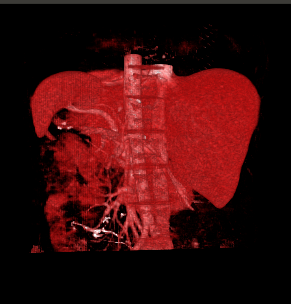
\includegraphics[trim= 0mm 0mm 0mm 0mm, clip, width=1.0\textwidth]{image/sl_0_2.png}}
	\end{columns}

	\setcounter{page}{0}
\end{frame}

%%%%%%%%%%%%%%%%%%%%%%%%%%%%%%%%%%%%%%%%%%%%%%%%%%%%%%%%%%%%%%%%%%%%%%%%%%%%%%% Section

\section{Introduction}

	\subsection[Presentation]{Presentation}
		\begin{frame}
			\frametitle{Presentation}			
			\begin{columns}[c]
			\column{25em}
				\begin{enumerate}
					\item Internship from March to July 2011
					\item Image analysis for diagnostic assistance
					\item Previous work: state of the art
					\item Programming language : Python 2.7
 				\end{enumerate}	
				\column{5em}
				\framebox{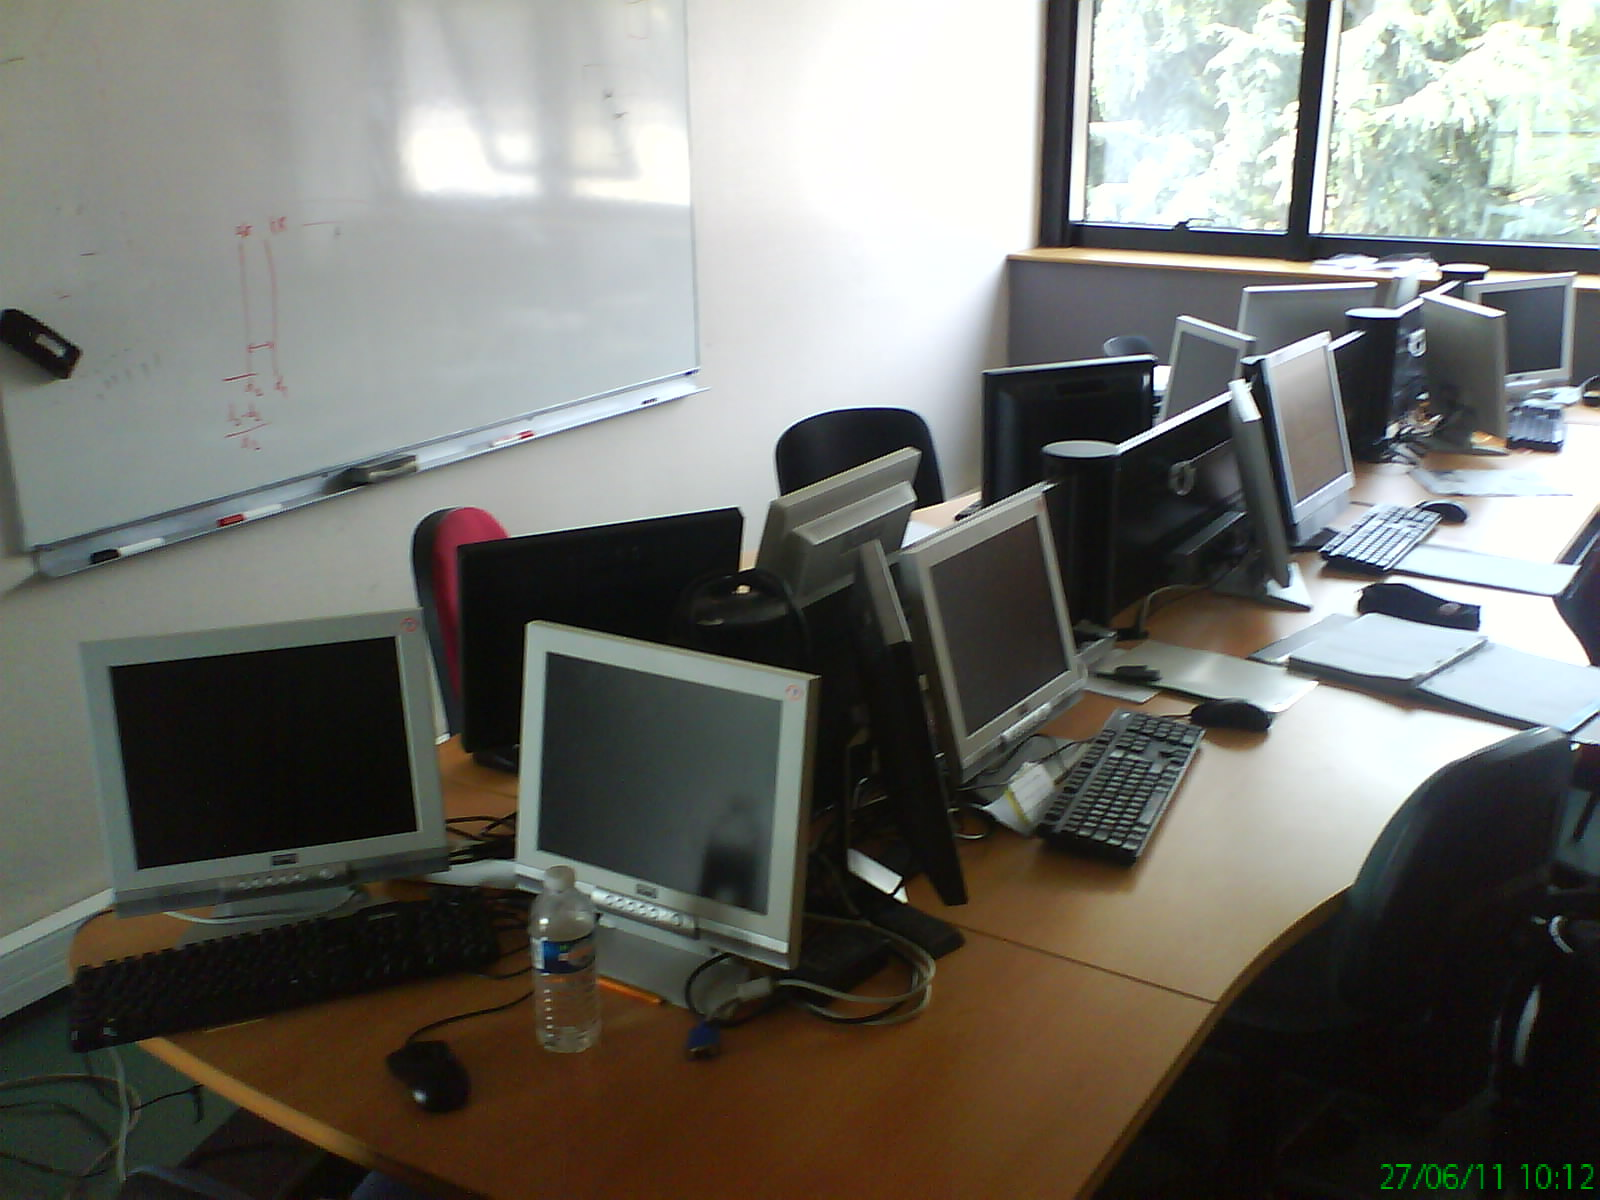
\includegraphics[trim= 0mm 0mm 0mm 0mm, clip, width=1.0\textwidth]{image/lisa_office.JPG}}\vspace{1em}
				\framebox{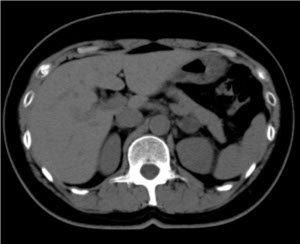
\includegraphics[trim= 0mm 0mm 0mm 0mm, clip, width=1.0\textwidth]{image/image_ct.jpg}}\vspace{1em}		
				\framebox{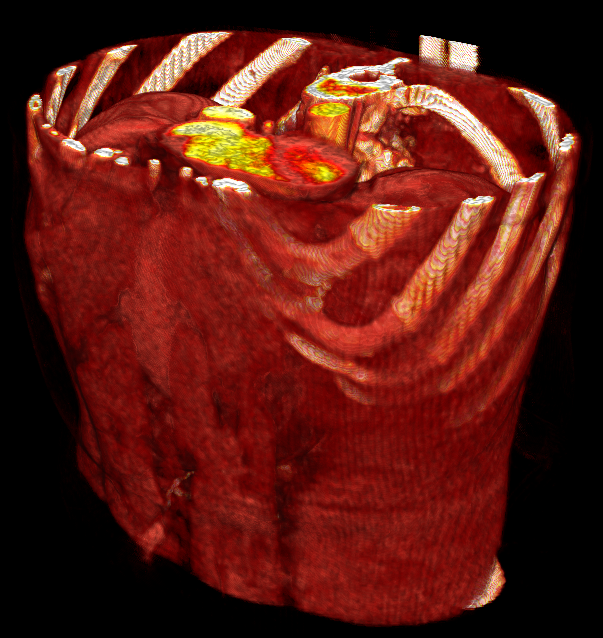
\includegraphics[trim= 0mm 0mm 0mm 0mm, clip, width=1.0\textwidth]{image/body.png}}
			\end{columns}
			\end{frame}

% * * * * * * * * * * * * * * * * * * * * * * * * * * * * * * * * * * * * * * * Slide

	\subsection[Understanding]{Image content understanding}
		\begin{frame}
		\frametitle{Image content understanding : sequential approach}
		%Initial image: 
		%a
		\begin{center}
			\framebox{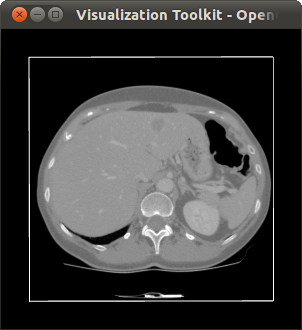
\includegraphics[trim= 10mm 15mm 10mm 28mm, clip, width=0.2\textwidth]{image/int_0_0_0}}\\
%			$\Downarrow$\\
%			\framebox(40,10){Segmentation}\\
			$\swarrow \downarrow \searrow$\\
			\line(1,0){100}\\
			
			\begin{columns}[c]
				\column{6em}
					\begin{center}
						\framebox{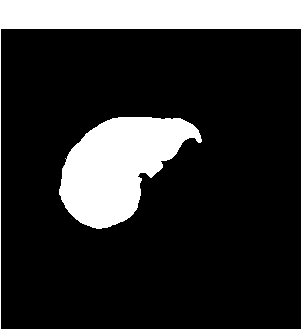
\includegraphics[trim= 15mm 25mm 15mm 35mm, clip, width=1.0\textwidth]{image/int_0_1_2.png}}\vspace{1em}
						\framebox{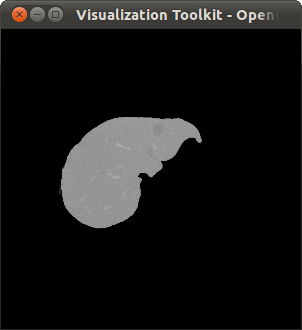
\includegraphics[trim= 15mm 25mm 15mm 35mm, clip, width=1.0\textwidth]{image/int_0_0_2.png}}\\
						$t=1$
					\end{center}
				\column{6em}
				\begin{center}
					\framebox{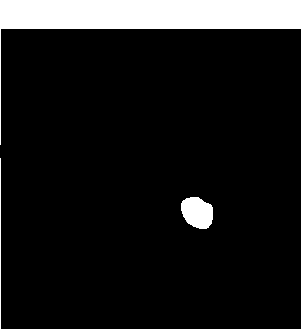
\includegraphics[trim= 15mm 25mm 15mm 35mm, clip, width=1.0\textwidth]{image/int_0_1_3.png}}\vspace{1em}
					\framebox{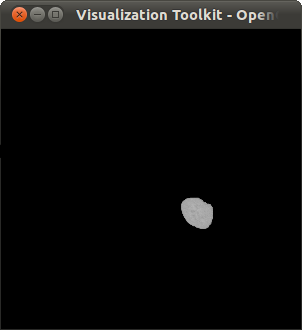
\includegraphics[trim= 15mm 25mm 15mm 35mm, clip, width=1.0\textwidth]{image/int_0_0_3.png}}\\
					$t=2$
				\end{center}
				\column{6em}
				\begin{center}
					\framebox{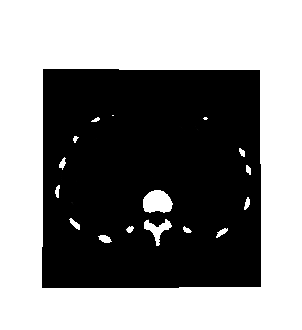
\includegraphics[trim= 15mm 25mm 15mm 35mm, clip, width=1.0\textwidth]{image/int_0_1_4.png}}\vspace{1em}
					\framebox{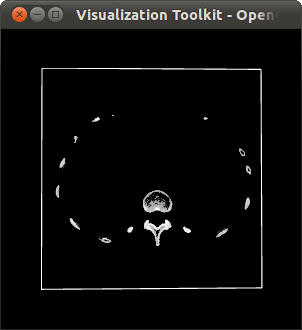
\includegraphics[trim= 15mm 25mm 15mm 35mm, clip, width=1.0\textwidth]{image/int_0_0_4.png}}\\
					$t=3$
				\end{center}
				\column{6em}
				\begin{center}
					\framebox{
\includegraphics[trim= 15mm 24mm 15mm 35mm, clip, width=1.0\textwidth]{image/int_0_1_6.png}}\vspace{1em}
					\framebox{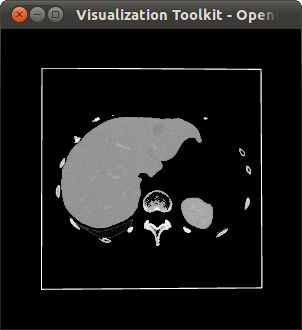
\includegraphics[trim= 15mm 24mm 15mm 35mm, clip, width=1.0\textwidth]{image/int_0_0_6.png}}\\
					%\framebox{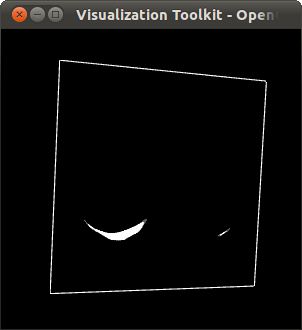
\includegraphics[trim= 20mm 25mm 20mm 35mm, clip, width=1.0\textwidth]{image/int_0_0_5.png}}\\
					Union
				\end{center}
			\end{columns}
			%$\searrow \downarrow \swarrow $	\\		
			%Final image: \framebox{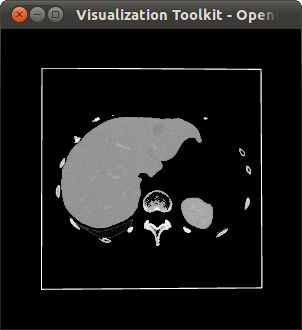
\includegraphics[trim= 15mm 20mm 15mm 30mm, clip, width=0.25\textwidth]{image/int_0_0_6.png}}
		\end{center}			
		
		\end{frame}
		
% * * * * * * * * * * * * * * * * * * * * * * * * * * * * * * * * * * * * * * * Slide

	\subsection[Problem]{Problem statement}
		\begin{frame}
		\frametitle{Problem statement}

%		\begin{columns}[c]
%		\column{25em}
			\begin{block}{How to represent and use non quantitative informations for image content understanding?}
				\begin{enumerate}
					\item e.g. vessels are not included in bones $\Rightarrow$ topology
					\item e.g. vessels are more bright than liver $\Rightarrow$ photometry
				\end{enumerate}

			\end{block}
%		\column{10em}
%			\framebox{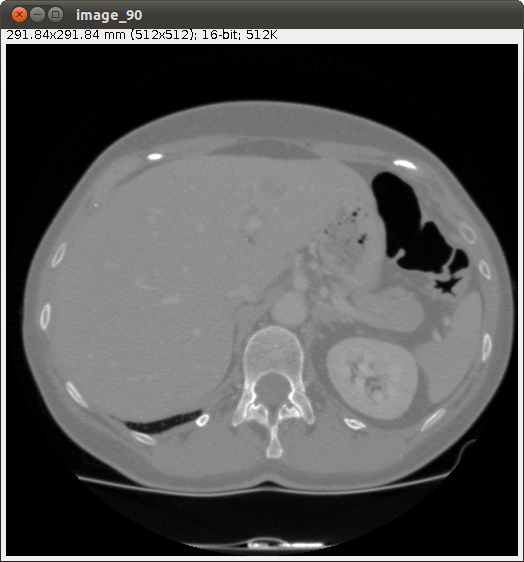
\includegraphics[trim= 5mm 15mm 3mm 25mm, clip, height=0.6\textwidth]{image/dicom.png}}
%		\end{columns}
		
		\vspace{1em}	
		
		\begin{columns}[c]
		\column{10em}
			\framebox{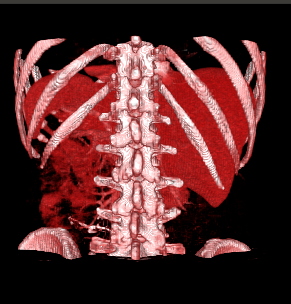
\includegraphics[trim= 0mm 0mm 0mm 0mm, clip, width=1.0\textwidth]{image/sl_0_1.png}}\vspace{1em}
			\framebox{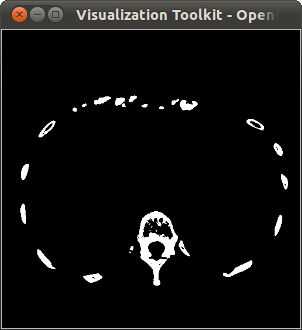
\includegraphics[trim= 0mm 0mm 0mm 20mm, clip, width=0.5\textwidth]{image/mask_bone}}
			\column{0.1em}
			$\Rightarrow$
			\column{10em}
			\framebox{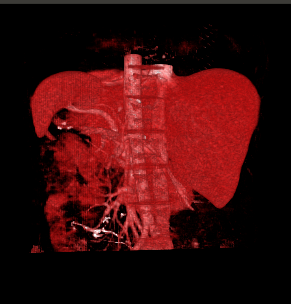
\includegraphics[trim= 0mm 0mm 0mm 0mm, clip, width=1.0\textwidth]{image/sl_0_2.png}}\vspace{1em}
			\framebox{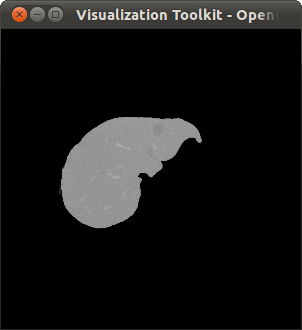
\includegraphics[trim= 10mm 10mm 10mm 30mm, clip, width=0.5\textwidth]{image/int_0_0_2}}			
			\column{0.1em}
			$\Rightarrow$
			\column{10em}
			\framebox{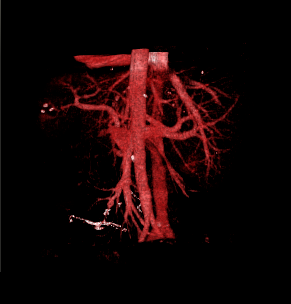
\includegraphics[trim= 0mm 0mm 0mm 0mm, clip, width=1.0\textwidth]{image/sl_0_3.png}}\vspace{6.5em}
		\end{columns}

		\end{frame}

% * * * * * * * * * * * * * * * * * * * * * * * * * * * * * * * * * * * * * * * Slide

	\subsection[State of the art]{State of the art}
		\begin{frame}
		\frametitle{What about state of the art?}
		
		\begin{block}{Image interpretation with a priori conceptual knowledges}

				Example : topological (e.g A include B), relative distance (e.g. A close to B), relative position (e.g. A is left to B)
%					\begin{enumerate}
%						\item[-] Topological (e.g A include B), relative distance (e.g. A close to B), relative position (e.g. A is left to B)
%					\end{enumerate}
			\begin{enumerate}
				\item Not common in image interpretation
				\item Nature
				\begin{enumerate}
					\item[-] Quantitative (e.g. distance, intensity)\footnotemark[1]
					\item[-] Non quantitative (e.g. inclusion, intersection)\footnotemark[2]
				\end{enumerate}
				\item Representation as graph\footnotemark[3]
				\begin{enumerate}
					\item[-] Contextual addition : active node\footnotemark[2]		%	Quantitative (e.g. distance, intensity)\footnotemark[1]
%					\item[-] Non quantitative (e.g. inclusion, intersection)\footnotemark[2]
%				\end{enumerate}				
%				\item Contextual addition
%				\begin{enumerate}
%					\item[-] Principle of active node\footnotemark[2]		
%					%\item[-] Non quantitative (e.g. inclusion, covering) \cite[Fasquel - 2006]{Fasquel2006}
				\end{enumerate}				
%				\item Conceptual graph representation\cite{deruyver2009}
			\end{enumerate}
			
		\end{block}
		
		 \footnotetext[1]{ \tiny \cite{Hudelot2008} C. Hudelot, J. Atif, and I. Bloch, Fuzzy spatial relation ontology for image interpretation, \emph{Fuzzy Sets and Systems}, 2008}
		 \footnotetext[2]{ \tiny \cite{Fasquel2006} J.-B. Fasquel, V. Agnus, An interactive medical image segmentation system based on the optimal management of regions of interest, \emph{Computer Methods and Programs in Biomedicine}, 2006}
		 \footnotetext[3]{ \tiny \cite{deruyver2009} A. Deruyver, Y. Hodéb, and L. Brun, Image interpretation with a conceptual graph, \emph{Artificial Intelligence}, 2009}
		
%		\begin{block}{Contextual information}
%			\begin{enumerate}
%				\item Adaptavive and specific to the image
%				\item Principle of active node \cite[Fasquel - 2006]{Fasquel2006}		
%			\end{enumerate}
%		\end{block}
		
		\begin{alertblock}{Contribution}
			Sequential approach with topological and photometrical knowledges.
		\end{alertblock}\vspace{1em}

%		\begin{columns}[c]		
%		\column{10em}
%			\framebox{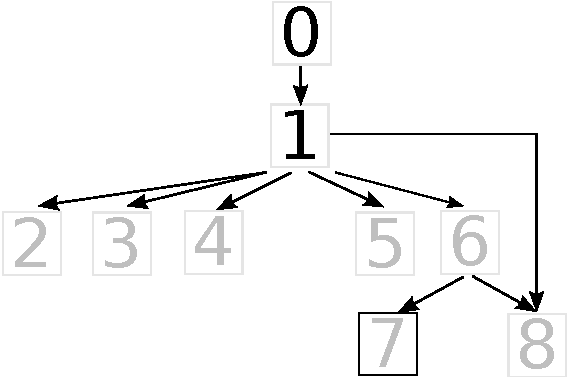
\includegraphics[trim= 0mm 0mm 0mm 0mm, clip, width=0.5\textwidth]{image/im_1_1_gt_0_tumor.pdf}}
%			\column{0.1em}
%			\column{10em}
%			\framebox{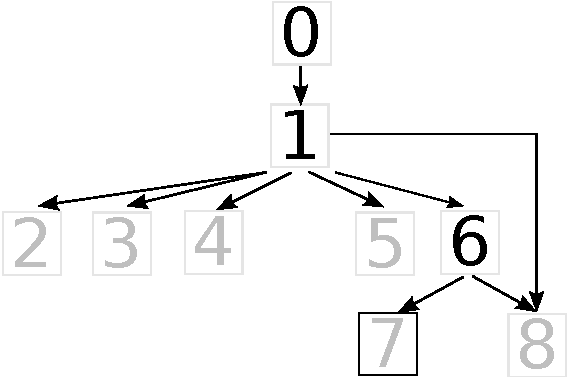
\includegraphics[trim= 0mm 0mm 0mm 0mm, clip, width=0.5\textwidth]{image/im_1_1_gt_1_tumor.pdf}}
%			\column{0.1em}
%			\column{10em}
%			\framebox{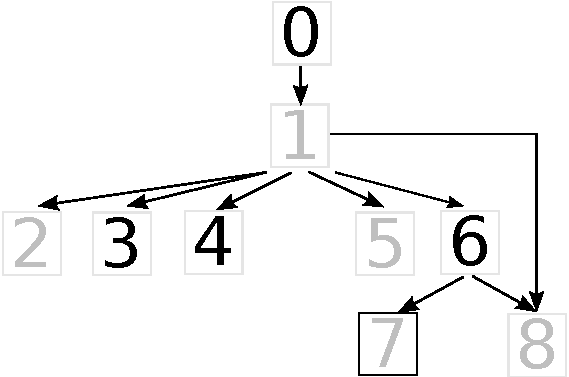
\includegraphics[trim= 0mm 0mm 0mm 0mm, clip, width=0.5\textwidth]{image/im_1_1_gt_2_tumor.pdf}}
%		\end{columns}


		
		\end{frame}

% * * * * * * * * * * * * * * * * * * * * * * * * * * * * * * * * * * * * * * * Slide

	\subsection[Steps]{Steps}	% Il est difficile de relier des informations de haut niveau et de bas niveau
		\begin{frame}
			\frametitle{Steps}
					\begin{columns}[c]
						\column{24em}
							\begin{block}{Representation}
								\begin{enumerate}
									\item Knowledge (conceptual information)
									\item Segmentation process (contextual information)
								\end{enumerate}		
							\end{block}							
							\begin{block}{Formalization (inference engine)}
								\begin{enumerate}
									\item Region of interest (topology)
									\item Number of classes (photometry)
									\item Class ordering (photometry)
								\end{enumerate}		
							\end{block}											
%							\begin{block}{Image}
%								\begin{enumerate}
%									\item Masking, clustering, windowing
%								\end{enumerate}		
%							\end{block}																
						
					\end{columns}

						\begin{columns}[c]
						\column{17em}				
							\begin{alertblock}{Evaluation}
								\begin{enumerate}
									\item Synthetic images
									\item Clustering algorithm
									\item Method's benefits quantification
								\end{enumerate}	
							\end{alertblock}																							
						\column{17em}				
							\begin{alertblock}{Application}
								\begin{enumerate}
									\item Medical images						
									\item Cluster identification
									\item Windowing for volume rendering
								\end{enumerate}	
							\end{alertblock}																							
					\end{columns}
%					\vspace{3em}
%						\alert{Validation from synthetic images to medical images. \\ADD FIGURE OF FULL PROCESS??}
												

						
%							\begin{block}{To do list}
%								\begin{enumerate}
%									\item Representation of conceptual informations
%									\item Modeling of thresholding process
%									\item Formalization of inference engine
%									\item Setting of thresholding algorithms
%								\end{enumerate}		
%							\end{block}



		\end{frame}

%%%%%%%%%%%%%%%%%%%%%%%%%%%%%%%%%%%%%%%%%%%%%%%%%%%%%%%%%%%%%%%%%%%%%%%%%%%%%%% Section

\section{Knowledge representation}
	\subsection[Topology \& photometry]{Topology \& photometry}
	\begin{frame}
		\frametitle{Topology \& photometry (conceptual informations)}
		\begin{block}{Graph}
			%Graphical representation of topologic and photometric relations between all the regions of an image :
			\begin{enumerate}
				\item Nodes are regions (e.g 0, 1, A, B, liver, tumor)
				\item Edges are relations (e.g. include, less bright than)
			\end{enumerate}					
		\end{block}
		\begin{columns}[c]
			\column{10em}		
				\begin{center}
					\framebox{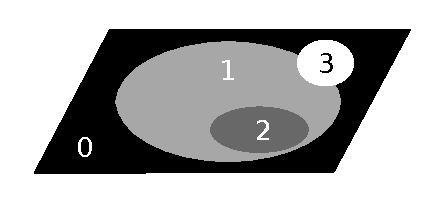
\includegraphics[trim= 0mm 0mm 0mm 0mm, clip, width=1.0\textwidth]{image/abc_img.pdf}}\\
				\end{center}	

			\column{10em}	
				\begin{exampleblock}{Topology}
					\begin{center}
						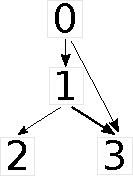
\includegraphics[trim= 0mm 0mm 0mm 0mm, clip, height=0.6\textwidth]{image/abc_graph_topo.pdf}
					\end{center}
				\end{exampleblock}
			\column{10em}
				\begin{exampleblock}{Photometry}
				\begin{center}
					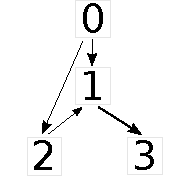
\includegraphics[trim= 0mm 0mm 0mm 0mm, clip, height=0.6\textwidth]{image/abc_graph_photo.pdf}
					\vspace{1em}
					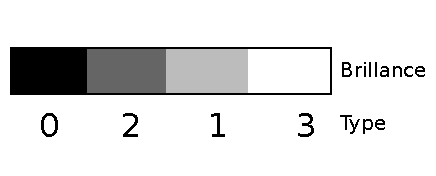
\includegraphics[trim= 0mm 0mm 17mm 0mm, clip, height=0.3\textwidth]{image/abc_graph_photo_gradient.pdf}
				\end{center}

				\end{exampleblock}
					
		\end{columns}	
	\end{frame}
	
% * * * * * * * * * * * * * * * * * * * * * * * * * * * * * * * * * * * * * * * Slide

\subsection[Segmentation process]{Segmentation process}
	\begin{frame}
		\frametitle{Segmentation process modeling (contextual informations)}
		\begin{block}{Add contextual information to the previous graph}
					\begin{enumerate}
						\item Active node = type is segmented
						\item Non active node = type is not segmented
					\end{enumerate}					
				\end{block}	
		\begin{columns}[c]
		
			\column{6em}<1->			
				\begin{exampleblock}{Date $t=0$}
					\begin{center}	
						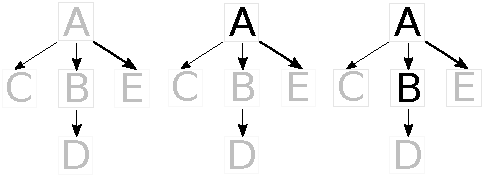
\includegraphics[trim= 0mm 0mm 57mm 0mm, clip, height=0.7\textwidth]{image/contex_gt.pdf}	\vspace{1em}
						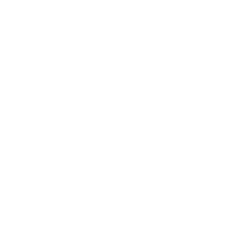
\includegraphics[trim= 0mm 0mm 0mm 0mm, clip, height=0.7\textwidth]{image/me_1_3_img_5.png}	\\
						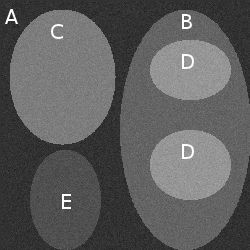
\includegraphics[trim= 0mm 0mm 0mm 0mm, clip, height=0.7\textwidth]{image/me_1_3_img_0.png}						
					\end{center}
				\end{exampleblock}
			\column{0.1em}<2->		
				A\\		
				$\Rightarrow$
			\column{6em}
				\begin{exampleblock}{Date $t=1$}<2->
					\begin{center}
						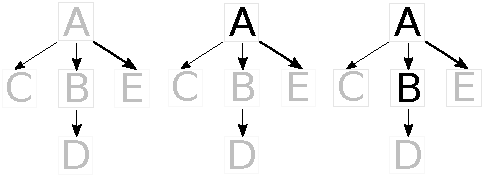
\includegraphics[trim= 28mm 0mm 28mm 0mm, clip, height=0.7\textwidth]{image/contex_gt.pdf}	\vspace{1em}
						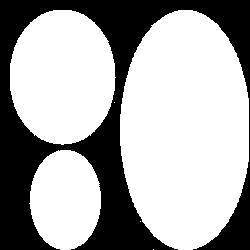
\includegraphics[trim= 0mm 0mm 0mm 0mm, clip, height=0.7\textwidth]{image/me_1_3_img_6.png}	\\%\vspace{1em}
						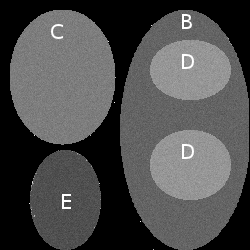
\includegraphics[trim= 0mm 0mm 0mm 0mm, clip, height=0.7\textwidth]{image/me_1_3_img_1.png}						
					\end{center}
				\end{exampleblock}
			\column{0.1em}<3->
				B\\			
				$\Rightarrow$
			\column{6em}
				\begin{exampleblock}{Date $t=2$}<3->
					\begin{center}
						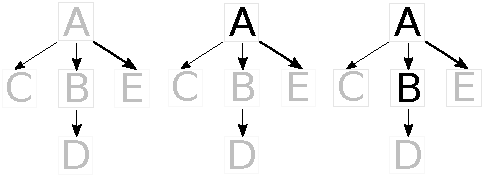
\includegraphics[trim= 56mm 0mm 0mm 0mm, clip, height=0.7\textwidth]{image/contex_gt.pdf}	\vspace{1em}					
						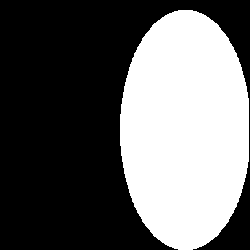
\includegraphics[trim= 0mm 0mm 0mm 0mm, clip, height=0.7\textwidth]{image/me_1_3_img_7.png}	\\
						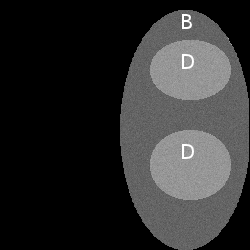
\includegraphics[trim= 0mm 0mm 0mm 0mm, clip, height=0.7\textwidth]{image/me_1_3_img_2.png}						
					\end{center}
				\end{exampleblock}

		\end{columns}
%		\vspace{2em}
%		\alert{Each segmented structure provides a mask that we apply on the original image.}
		
	\end{frame}	
	
%%%%%%%%%%%%%%%%%%%%%%%%%%%%%%%%%%%%%%%%%%%%%%%%%%%%%%%%%%%%%%%%%%%%%%%%%%%%%%% Section

\section[Engine]{Inference engine}
%	\subsection[Presentation]{Presentation}
%	\begin{frame}
%			\frametitle{Presentation}
%			\alert{Mixing conceptual and contextual informations}
%	\end{frame}
	\subsection[ROI]{Region Of Interest}
		\begin{frame}
			\frametitle{From the optimal region of interest...}
			\begin{block}{Optimal Region Of Interest\footnotemark[1]}

				%%%%%%%%%%%%%%%%%%%%%%%%%%%%%%%%%%%%%%%%%%%%%%%%%%%
				\begin{equation}
					R_t(u)=\left(\bigcup_{l\in G_{T,t}^{-1}(u)}X_t(\overline{l})\right) \cup \left(\bigcup_{i\in S_t| u\in G_{T,t}^{-\infty}(i)}X_t(i) \right)
				\end{equation}
				%%%%%%%%%%%%%%%%%%%%%%%%%%%%%%%%%%%%%%%%%%%%%%%%%%%
			\end{block}

			\begin{exampleblock}{Example}
				\begin{columns}[c]
					\column{5em}
					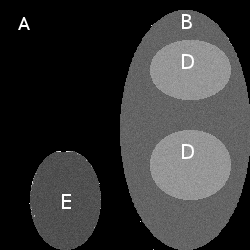
\includegraphics[trim= -5mm 0mm 0mm 0mm, clip, height=1\textwidth]{image/lobe_img.png}
%					\column{5em}
%					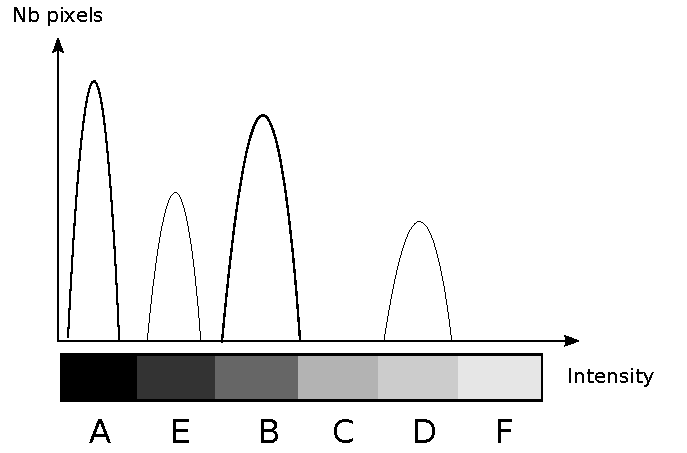
\includegraphics[trim= -5mm 0mm 0mm 0mm, clip, height=1.2\textwidth]{image/lobe_hist.pdf}
					\column{5em}
					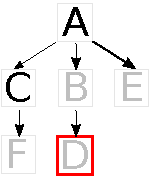
\includegraphics[trim= -5mm 0mm 0mm 0mm, clip, height=1\textwidth]{image/roi_gt.pdf}
				\end{columns}
			\end{exampleblock}

			\begin{columns}[c]	
				\column{15em}			
					\begin{alertblock}{ROI}
						$ R_t(D) = X_t(\bar{A}) $\\
						$ R_t(D) = X_t(A) \setminus X_t(C)$\\
						%$ N_t(D) = 4$

					\end{alertblock}
					
			\end{columns}
		 	\footnotetext[1]{ \cite{Fasquel2006} J.-B. Fasquel, V. Agnus, \emph{Computer Methods and Programs in Biomedicine}, 2006}				
		\end{frame}
		
% * * * * * * * * * * * * * * * * * * * * * * * * * * * * * * * * * * * * * * * Slide

	\subsection[Number of lobes]{Number of classes}
		\begin{frame}
			\frametitle{... to the number of classes}
			\begin{block}{List of classes $\Leftrightarrow$ lobes in the histogram}
				%%%%%%%%%%%%%%%%%%%%%%%%%%%%%%%%%%%%%%%%%%%%%%%%%%%
				\begin{equation}
			 	  	L_t(u) = \Big\{ i \in \left( G_T^{\infty}(G_{T,t}^{-1} (u)) \cap ( S \setminus S_t ) \right) \;|\; \left( G_{T,t}^{-1} (i) \cap G_{T,t}^{-1} (u) \neq \emptyset \right) \Big\} \cup  G_{T,t}^{-1}(u)
				\end{equation}
			 	%%%%%%%%%%%%%%%%%%%%%%%%%%%%%%%%%%%%%%%%%%%%%%%%%%%
			\end{block}			

			\begin{exampleblock}{Example}
				\begin{columns}[c]
					\column{5em}
					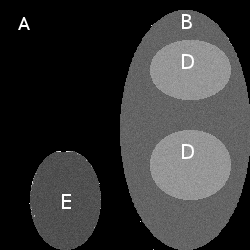
\includegraphics[trim= -5mm 0mm 0mm 0mm, clip, height=1\textwidth]{image/lobe_img.png}
					\column{5em}
					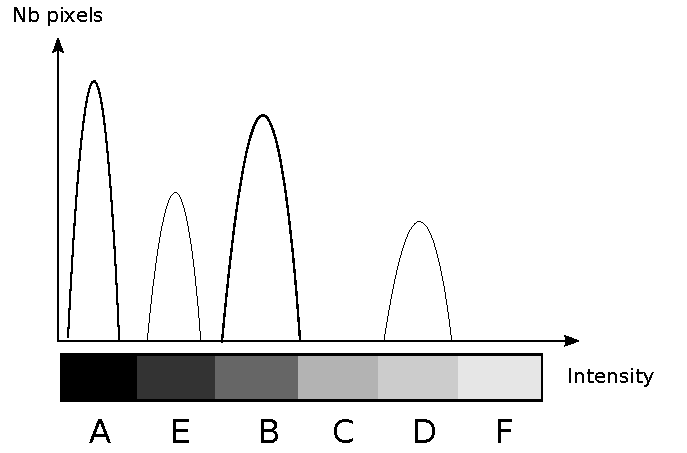
\includegraphics[trim= -5mm 0mm 0mm 0mm, clip, height=1.2\textwidth]{image/lobe_hist.pdf}
					\column{5em}
					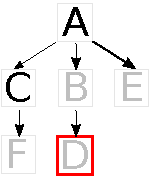
\includegraphics[trim= -5mm 0mm 0mm 0mm, clip, height=1\textwidth]{image/roi_gt.pdf}
%					\column{5em}
%					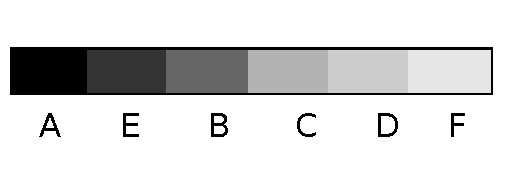
\includegraphics[trim= 0mm 0mm 0mm 0mm, clip, width=1\textwidth]{image/ident_gp.pdf}
					%\hspace{3em}$L_t(D) = \big\{ B, E, D$\hspace{1.35em}| \hspace{5.5em} $\emptyset$\hspace{4.em}\big\}\;$ \cup \;\;\;A$\\
					%\hspace{3em}$L_t(D) = A,B,E,D$
				\end{columns}
			\end{exampleblock}

			\begin{columns}[c]	
				\column{18em}			

				\begin{alertblock}{Cardinality}
					A priori number of classes in the ROI:
					$ N_t(u) = \left|{L_t(u)}\right|$\\
					$ N_t(D) = \left|{L_t(D)}\right| = \left|{B,E,D,A}\right|$\\
					$ N_t(D) = 4$

				\end{alertblock}
				
%				\begin{center}	
%					\framebox{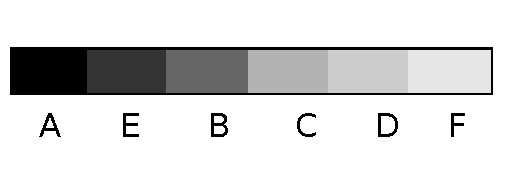
\includegraphics[trim= 0mm 0mm 0mm 0mm, clip, height=0.2\textwidth]{image/ident_gp.pdf}}
%				\end{center}

				\column{15em}	
				\begin{alertblock}{Identification}
				Ordering by photometry: % and \alert{identification}:
				$O_t(u) = \operatorname{ord} \{ L_t(u) \}$
				%$O_t(D) = \operatorname{ord} \{ L_t(D) \}$
				$O_t(D) = \operatorname{ord} \{ B,E,D,A \}$
				$O_t(D) = \{ A, E, B, D \}$
				
				\end{alertblock}					
			\end{columns}


		\end{frame}
		

% * * * * * * * * * * * * * * * * * * * * * * * * * * * * * * * * * * * * * * * Slide

	\subsection[Results]{Results}
		\begin{frame}
			\frametitle{Results}
			\begin{block}{Conclusion}
				\begin{enumerate}
					\item Not easy as it seems
					\item Limit of the study for the number of classes
					\begin{enumerate}
						\item[-] Segmentation of a type in once $\Rightarrow$ no multiplicity
						\item[-] Types are all in the image $\Rightarrow$ no optionality
						%\item Total inclusion (e.g. )
					\end{enumerate}

				\end{enumerate}
			\end{block}			
		\end{frame}
		


		
% * * * * * * * * * * * * * * * * * * * * * * * * * * * * * * * * * * * * * * * Slide


% * * * * * * * * * * * * * * * * * * * * * * * * * * * * * * * * * * * * * * *
% * * * * * * * * * * * * * * * * * * * * * * * * * * * * * * * * * * * * * * *	

